\section {Конечные автоматы. Регулярные языки}
\subsection{Детерминированные конечные автоматы}
\begin{conj}
    Детерминированный конечный автомат.\\
    $\Sigma$ - конечный алфавит\\
    $Q$ - конечное множество состояний.\\
    $q_o \in Q$ - начальное состояние\\
    $F \subseteq Q$ - множество конечных состояний\\
    $\delta : Q \times \Sigma \to Q$ - переходы\\
    На вход подаётся строка $x \in \Sigma^*$, то есть $x = x_1x_2\dots x_n,\ x_i \in \Sigma,\ n \geq 0$\\
    В процессе работы автомат принимает состояния $q_{i_1}, q_{i_2}, \dots, q_{i_n}$\\
    $q_{i_1} = \delta(q_0, x_1)$\\
    $q_{i_2} = \delta(q_{i_1}, x_2)$\\
    $\vdots$\\
    $q_i{n} = \delta(q_{i_{n-1}}, x_n)$\\
    Автомат принимает строку $x$, если $q_{i_n} \in F$, иначе отвергает
\end{conj}

\begin{conj}
    Язык $L$ называется регулярным, если $\exists$ ДКА $A : \forall x\ x \in L \Leftrightarrow A$ принимает x.
\end{conj}

\textbf{Примеры}
\begin{enumerate}
    \item $\Sigma = \{\text{a, b, c, }\dots \text{, z}\}$\\
    $L$ - множество всех строк, содержащих подстроку $mkn$



    \tikzset{every picture/.style={line width=0.75pt}} %set default line width to 0.75pt        

    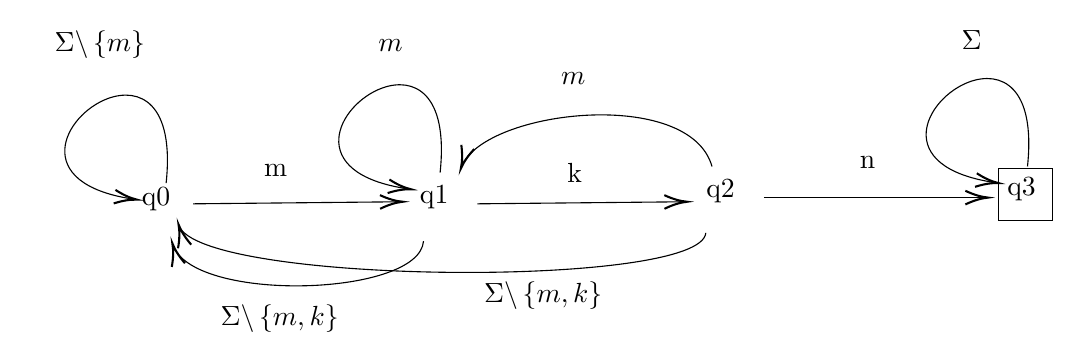
\begin{tikzpicture}[x=0.75pt,y=0.75pt,yscale=-1,xscale=1]
    %uncomment if require: \path (0,300); %set diagram left start at 0, and has height of 300
    
    %Straight Lines [id:da03667137013515909] 
    \draw    (113,138) -- (212,137.02) ;
    \draw [shift={(214,137)}, rotate = 179.43] [color={rgb, 255:red, 0; green, 0; blue, 0 }  ][line width=0.75]    (10.93,-3.29) .. controls (6.95,-1.4) and (3.31,-0.3) .. (0,0) .. controls (3.31,0.3) and (6.95,1.4) .. (10.93,3.29)   ;
    %Straight Lines [id:da6180334490030455] 
    \draw    (250,138) -- (349,137.02) ;
    \draw [shift={(351,137)}, rotate = 179.43] [color={rgb, 255:red, 0; green, 0; blue, 0 }  ][line width=0.75]    (10.93,-3.29) .. controls (6.95,-1.4) and (3.31,-0.3) .. (0,0) .. controls (3.31,0.3) and (6.95,1.4) .. (10.93,3.29)   ;
    %Straight Lines [id:da011510213933319413] 
    \draw    (388,135) -- (494,135) ;
    \draw [shift={(496,135)}, rotate = 180] [color={rgb, 255:red, 0; green, 0; blue, 0 }  ][line width=0.75]    (10.93,-3.29) .. controls (6.95,-1.4) and (3.31,-0.3) .. (0,0) .. controls (3.31,0.3) and (6.95,1.4) .. (10.93,3.29)   ;
    %Curve Lines [id:da42936903875876253] 
    \draw    (100,128) .. controls (104.13,89.13) and (87.07,81.72) .. (71.99,87.25) .. controls (50.82,95.01) and (33.56,128.29) .. (84.44,135.78) ;
    \draw [shift={(86,136)}, rotate = 187.59] [color={rgb, 255:red, 0; green, 0; blue, 0 }  ][line width=0.75]    (10.93,-3.29) .. controls (6.95,-1.4) and (3.31,-0.3) .. (0,0) .. controls (3.31,0.3) and (6.95,1.4) .. (10.93,3.29)   ;
    %Curve Lines [id:da2988940358511245] 
    \draw    (232,123) .. controls (236.13,84.13) and (219.07,76.72) .. (203.99,82.25) .. controls (182.82,90.01) and (165.56,123.29) .. (216.44,130.78) ;
    \draw [shift={(218,131)}, rotate = 187.59] [color={rgb, 255:red, 0; green, 0; blue, 0 }  ][line width=0.75]    (10.93,-3.29) .. controls (6.95,-1.4) and (3.31,-0.3) .. (0,0) .. controls (3.31,0.3) and (6.95,1.4) .. (10.93,3.29)   ;
    %Curve Lines [id:da7176695089660099] 
    \draw    (515,120) .. controls (519.13,81.13) and (502.07,73.72) .. (486.99,79.25) .. controls (465.82,87.01) and (448.56,120.29) .. (499.44,127.78) ;
    \draw [shift={(501,128)}, rotate = 187.59] [color={rgb, 255:red, 0; green, 0; blue, 0 }  ][line width=0.75]    (10.93,-3.29) .. controls (6.95,-1.4) and (3.31,-0.3) .. (0,0) .. controls (3.31,0.3) and (6.95,1.4) .. (10.93,3.29)   ;
    %Shape: Rectangle [id:dp7359991183192658] 
    \draw   (501,121) -- (527,121) -- (527,146) -- (501,146) -- cycle ;
    %Curve Lines [id:da4112641807017492] 
    \draw    (224,156) .. controls (222.04,182.46) and (115.4,185.87) .. (103.6,158.7) ;
    \draw [shift={(103,157)}, rotate = 74.58] [color={rgb, 255:red, 0; green, 0; blue, 0 }  ][line width=0.75]    (10.93,-3.29) .. controls (6.95,-1.4) and (3.31,-0.3) .. (0,0) .. controls (3.31,0.3) and (6.95,1.4) .. (10.93,3.29)   ;
    %Curve Lines [id:da04521522971228631] 
    \draw    (360,152) .. controls (358.04,178.46) and (123.66,177.07) .. (106.76,149.71) ;
    \draw [shift={(106,148)}, rotate = 74.58] [color={rgb, 255:red, 0; green, 0; blue, 0 }  ][line width=0.75]    (10.93,-3.29) .. controls (6.95,-1.4) and (3.31,-0.3) .. (0,0) .. controls (3.31,0.3) and (6.95,1.4) .. (10.93,3.29)   ;
    %Curve Lines [id:da9223063895210342] 
    \draw    (363,120) .. controls (352.22,81.78) and (255,92.54) .. (242.65,119.34) ;
    \draw [shift={(242,121)}, rotate = 287.82] [color={rgb, 255:red, 0; green, 0; blue, 0 }  ][line width=0.75]    (10.93,-3.29) .. controls (6.95,-1.4) and (3.31,-0.3) .. (0,0) .. controls (3.31,0.3) and (6.95,1.4) .. (10.93,3.29)   ;
    
    % Text Node
    \draw (87,129) node [anchor=north west][inner sep=0.75pt]   [align=left] {q0};
    % Text Node
    \draw (221,128) node [anchor=north west][inner sep=0.75pt]   [align=left] {q1};
    % Text Node
    \draw (359,125) node [anchor=north west][inner sep=0.75pt]   [align=left] {q2};
    % Text Node
    \draw (504,124) node [anchor=north west][inner sep=0.75pt]   [align=left] {q3};
    % Text Node
    \draw (146,118) node [anchor=north west][inner sep=0.75pt]   [align=left] {m};
    % Text Node
    \draw (292,117) node [anchor=north west][inner sep=0.75pt]   [align=left] {k};
    % Text Node
    \draw (45,53.4) node [anchor=north west][inner sep=0.75pt]    {$\Sigma \backslash \left\{\text{m}\right\}$};
    % Text Node
    \draw (201,57.4) node [anchor=north west][inner sep=0.75pt]    {$\text{m}$};
    % Text Node
    \draw (125,185.4) node [anchor=north west][inner sep=0.75pt]    {$\Sigma \backslash \left\{\text{m, k}\right\}$};
    % Text Node
    \draw (482,53.4) node [anchor=north west][inner sep=0.75pt]    {$\Sigma $};
    % Text Node
    \draw (433,114) node [anchor=north west][inner sep=0.75pt]   [align=left] {n};
    % Text Node
    \draw (252,174.4) node [anchor=north west][inner sep=0.75pt]    {$\Sigma \backslash \left\{\text{m, k}\right\}$};
    % Text Node
    \draw (289,73.4) node [anchor=north west][inner sep=0.75pt]    {$\text{m}$};
    
    
    \end{tikzpicture}


    \item $\Sigma = \{0, 1\},\ L = \{x \in \{0, 1\}^n | \text{в } x \text{ нечетное число единиц}\}$

    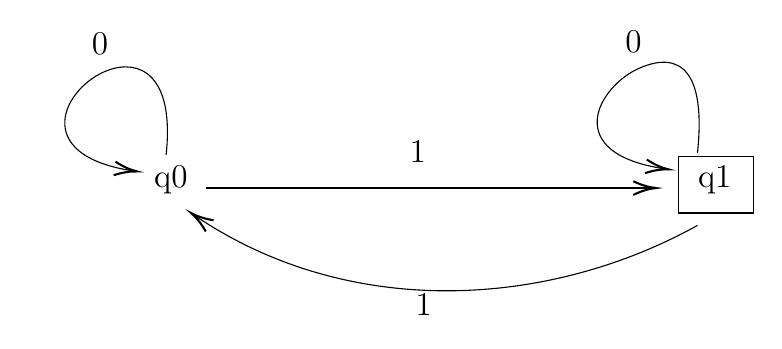
\begin{tikzpicture}[x=0.75pt,y=0.75pt,yscale=-1,xscale=1]
    %uncomment if require: \path (0,300); %set diagram left start at 0, and has height of 300

    %Shape: Rectangle [id:dp4677180275751667] 
    \draw   (376,139) -- (412,139) -- (412,166) -- (376,166) -- cycle ;
    %Curve Lines [id:da4709746404392907] 
    \draw    (129,138) .. controls (133.13,99.13) and (116.07,91.72) .. (100.99,97.25) .. controls (79.82,105.01) and (62.56,138.29) .. (113.44,145.78) ;
    \draw [shift={(115,146)}, rotate = 187.59] [color={rgb, 255:red, 0; green, 0; blue, 0 }  ][line width=0.75]    (10.93,-3.29) .. controls (6.95,-1.4) and (3.31,-0.3) .. (0,0) .. controls (3.31,0.3) and (6.95,1.4) .. (10.93,3.29)   ;
    %Curve Lines [id:da5017111880538947] 
    \draw    (385,137) .. controls (389.13,98.13) and (376.98,87.5) .. (356.99,96.25) .. controls (337.2,104.91) and (318.59,137.3) .. (369.44,144.78) ;
    \draw [shift={(371,145)}, rotate = 187.59] [color={rgb, 255:red, 0; green, 0; blue, 0 }  ][line width=0.75]    (10.93,-3.29) .. controls (6.95,-1.4) and (3.31,-0.3) .. (0,0) .. controls (3.31,0.3) and (6.95,1.4) .. (10.93,3.29)   ;
    %Straight Lines [id:da3636468810946405] 
    \draw    (148,154) -- (363,154) ;
    \draw [shift={(365,154)}, rotate = 180] [color={rgb, 255:red, 0; green, 0; blue, 0 }  ][line width=0.75]    (10.93,-3.29) .. controls (6.95,-1.4) and (3.31,-0.3) .. (0,0) .. controls (3.31,0.3) and (6.95,1.4) .. (10.93,3.29)   ;
    %Curve Lines [id:da2243912938130701] 
    \draw    (385,172) .. controls (313.36,211.8) and (216.97,217.94) .. (142.13,166.78) ;
    \draw [shift={(141,166)}, rotate = 34.73] [color={rgb, 255:red, 0; green, 0; blue, 0 }  ][line width=0.75]    (10.93,-3.29) .. controls (6.95,-1.4) and (3.31,-0.3) .. (0,0) .. controls (3.31,0.3) and (6.95,1.4) .. (10.93,3.29)   ;

    % Text Node
    \draw (122,142) node [anchor=north west][inner sep=0.75pt]   [align=left] {{\large q0}};
    % Text Node
    \draw (384,142) node [anchor=north west][inner sep=0.75pt]   [align=left] {{\large q1}};
    % Text Node
    \draw (92,78) node [anchor=north west][inner sep=0.75pt]   [align=left] {{\large 0}};
    % Text Node
    \draw (349,77) node [anchor=north west][inner sep=0.75pt]   [align=left] {{\large 0}};
    % Text Node
    \draw (245,130) node [anchor=north west][inner sep=0.75pt]   [align=left] {{\large 1}};
    % Text Node
    \draw (248,204) node [anchor=north west][inner sep=0.75pt]   [align=left] {{\large 1}};

    \end{tikzpicture}

    \item $\Sigma = \{0, 1\} L = \{0^n 1^n | n \in \mathbb{N}\}$ не является регулярным. 
    Важный пример, так как похожая идея позволяет доказать нерегулярность многих языков

    \begin{proof}
        От противного. Пусть есть ДКА $A$ на $k$ состояниях, который распознает этот язык. Рассмотрим строки 
        $0, 00, \dots, 0^{k+1}$. По принципу Дирихле $\exists i, j,\ i\neq j$, такие что $A(0^i)$ придет в то же состояние, что $A(0^j)$
        Но тогда $A(0^i 1^i)$ и $A(0^j 1^i)$ тоже придут в одно состояние (после нулей они в одном, а затем равное количество единиц). Но $0^i 1^i$ автомат должен принять, а $0^j 1^i$ не принять. Противоречие.
    \end{proof}

\end{enumerate}

\textbf{Операции над языками}
\begin{enumerate}
    \item Дополнение: $\overline L = \Sigma^* \setminus L$. Множество регулярных языков замкнуто относительно дополнения (чтобы автомат принимал дополнение языка, поменяем местами финальные и нефинальные состояния)
    \item Пересечение регулярных языков $L_1 \cap L_2$ - регулярный язык
    \item Объединение регулярных языков $L_1 \cup L_2$ - регулярный язык\\
    \begin{proof}
        Возьмем ДКА $(Q_1, q_0, F_1, \sigma_1)$ для языка $L_1$ и автомат $(Q_2, q_0', F_2, \sigma_2)$ для языка $L_2$.\\
        Тогда новый автомат будет в качестве состояний иметь все элементы $(Q_1 \times Q_2)$ с переходами $\sigma(q_1, q_2, c) = (\delta_1(q_1, c), \delta_2(q_2, c))$.\\
        Чтобы получить пересечение языков, в качестве конечных состояний надо взять $F_1 \times F_2$, для объединения $F_1 \times Q_2 \cup Q_1 \times F_2$
    \end{proof}
    \item Конкатенация $L_1 \circ L_2 = \{ xy | x \in L_1, y \in L2\}$
    \item Операция $*$: $L^* = \{x_1, \dots x_n | n \geq 0,\ x_i \in L\}$ (замыкание Клини)
\end{enumerate}


\subsection{Недетерминированне конечные автоматы}

\begin{conj}
    Недетерминированный конечный автомат (НКА)\\
    $\Sigma$ - конечный алфавит\\
    $Q$ - множество состояний\\
    $q_0 \in Q$ - начальное состояние\\
    $F \subseteq Q$ - конечные состояния
    $\delta: Q \times \Sigma \to 2^Q$\\
\end{conj}
\begin{conj}
    Корректное принимающее (принимаемое?) вычисление на входе $x$ для НКА, $x = x_1, \dots, x_n$\\
    $q_{i_1} \in \sigma(q_0, x_1)$\\
    $q_{i_2} \in \sigma (q_{i_1}, x_2)\\
    \vdots\\
    q_{i_n} \in \sigma (q_{i_{n-1}}, x_n)\\$
\end{conj}

НКА принимает строку $x$, если существует корректное принимающее вычисление.

Пояснение: в ДКА из каждого состояния могла идти только одна стрелка(переход) с каждым символом, поэтому у нас всегда ровно один путь, по которому можно пойти в процессе обработки фиксированного слова (поэтому автомат называется детерминированным).
В НКА из состояния может идти несколько стрелок с одинаковым символом. Если из определения не очевидно, то об этом можно думать двумя способами:

\begin{itemize}
    \item Когда существует путь до какой-либо финальной вершины, то автомат принимает строку. Если все возможные пути заканчиваются в не финальном состоянии, то не принимает.
    \item В случае, когда нужно пойти по одной из них, мы создаем столько копий автомата, сколько у нас стрелок, каждая пойдет по своему пути. 
Каждая из них будет создавать новые копии, если будет снова встречать возможность пойти по нескольким стрелкам. Процесс конечен, так как каждый раз мы откусываем по одному символу. Тогда если хоть одна копия дойдет до какого-либо финального состояния, автомат принимает строку.
\end{itemize}

\begin{conj}
    НКА с $\varepsilon$-переходами. $\Sigma_\varepsilon = \Sigma \cup \{\varepsilon\}$, $\delta : Q \times \varepsilon \to 2^Q$. 
    Автомат $A$ с $\varepsilon$ переходами принимает строку $x$, если $\exists x' \in \Sigma^*_\varepsilon$, такой что $x$ получается из $x'$ вычеркиванием $\varepsilon$ и 
    строка $x'$ принимается автоматом $A$ по правилам НКА.
\end{conj}

Другими словами, на некоторых стрелках(переходах) теперь написан не символ, а $\varepsilon$. Если мы идём по нему, то состояние изменяется согласно переходу, однако текущий символ не меняется. То есть $\varepsilon$-переход меняет состояние, не "съедая" символ. 
Заметим, что может оказаться, что по автомату теперь можно ходить бесконечно, но определение строго разрешает этот вопрос - если есть путь в финальное состояние, то слово принято, иначе нет.

\begin{theorem}
    ДКА, НКА и $\text{НКА}_\varepsilon$ распознают одно и то же множество языков
\end{theorem}

\begin{proof}
    $"\Leftarrow"$ - очевидно. ДКА является частным случаем НКА.
    $"\Rightarrow"$. Пусть есть НКА $\Sigma, Q, q_0, F, \delta : Q \times \Sigma \to 2^Q$ для L. Построим ДКА $A'$, у которого состояниями являются подмножества $Q:\ Q' \subset 2^Q$.\\
    $q'_0 = \{q_0\}$\\
    $F' = \{S \subset Q' | S \cap F \neq \varnothing$\\
    $\delta' : Q' \times \Sigma \to Q'$\\
    $\delta'(S, c) = \cup_{q \in S} \delta(q, c)$\\
    Доказательство становится очевидным после понимания утверждения - через $n$ шагов состояние $A'$ будет соответствовать множеству всех состояний $A$, до которых можно было добраться за $n$ шагов получив на входе слово $x$. 
    Это легко видеть например по индукции - база $q'_0$, переход по определению $\delta'$.
\end{proof}

\begin{theorem}
    НКА и $\text{НКА}_\varepsilon$ распознают одно и то же множество языков
\end{theorem}

\begin{proof}
    $"\Leftarrow"$ - очевидно.
    $"\Rightarrow"$ Для каждого состояния $q \in Q$ найдём множество состояний $S_q$ - достижимых из него только по $\varepsilon$-переходам.
    Теперь в любое состояние, в которое мы могли попасть хоть из одного $S_q$, мы должны уметь напрямую из $Q$. Формально сделаем так: 
    $\forall q' \in S_q\ \forall a \in \Sigma\ q'' \in \sigma(q', a) \Rightarrow$ добавим $q''$ в $\delta(q, a)$. Легко видеть, что мы построили эквивалентный автомат.
\end{proof}

ДКА, НКА, $\text{НКА}_\varepsilon$ задают множество регулярных языков\\

\textbf{Утверждение.} Множество регулярных языков замкнуто относительно конкатенации и $*$

\begin{proof}
    Конкатенация: сделаем автомат для первого языка, из его финальных состояний добавим $\varepsilon$-переходы в начальное состояние автомата для второго языка.\\
    Замыкание Клини: сделаем $\varepsilon$ переходы из финальных состояний в своё начальное.\\

    Может быть неочевидно, почему мы случайно не распознаем какие-то лишние слова, ведь мы обрабатывали какое-то слово, а посередине могли прыгнуть в какой-то другой автомат или в своё начало. Но если состояние помечено как финальное и мы в него пришли в результате обработки какого-то префикса $x_1, \dots x_k$ строки $x$ длины $n > k$, то слово $x_1, \dots x_k$ тоже лежит в языке.
\end{proof}

\subsection{Регулярные выражения}
\begin{conj}
    Синтаксис регулярных выражений над алфавитом $\Sigma$
    \begin{itemize}
        \item Буква из $\Sigma$ - это регулярное выражение
        \item $\Lambda и \varepsilon$ - регулярные выражения
        \item $A_1, A_2, \dots, A_n$ - регулярные выражения. Тогда $A_1 | A_2 \dots | A_n$ - регулярные выражения
        \item $A_1, \dots, A_n$ - регулярные выражения. Тогда $(A_1 A_2 \dots A_n)$ - регулярные выражения
        \item $A$ - регулярное выражения, тогда $A^*$ регулярное выражение.
    \end{itemize}

    Семантика регулярных выражений: 
    \begin{itemize}
        \item Регулярное выражение $\Leftrightarrow$ язык в алфавите $\varepsilon$.
        \item $a \in \Sigma$ - $\{a\}$
        \item $\varepsilon \in \Sigma$ - пустой язык ($\varnothing$)
        \item $\Lambda \in \Sigma - \{\varepsilon\}$ - язык из пустого слова 
        \item $A_1, \dots A_n$ соответствуют языкам $L_1, \dots, L_n$. Тогда $A_1 | A_2 \dots | A_n$ соответствует языку $L_1 \cup L_2 \cup \dots \cup L_n$
        \item $A_1 A_2 \dots A_n$ соответствует $L_1 \circ L_2 \circ \dots \circ L_n$
        \item $A^*$ соотвествует $L^*$
    \end{itemize}
\end{conj}

\begin{theorem}
    Язык $L$ регулярен $\Leftrightarrow L$ задается регулярным выражением.
\end{theorem}

\begin{proof}
    $"\Leftarrow"$ Следует из того, что множество регулярных языков замкнуто относительно всех этих операций ($\cup$, конкатенация, $*$)
    $"\Rightarrow"$ Строим регулярное выражение по конечному автомату, удобнее по НКА, так как его можно переделать, чтобы финальное состояние было только одно.\\
    Пусть язык $L$ задан НКА с единственным конечным состоянием. $q_1$ - начальное, $q_k$ - конечное. $Q = \{q_1, q_2, \dots, q_k\}$.\\
    $D_{i,j,s}$ - множество таких слов, что из $q_i$ можно прочитав эти слова прийти в $q_j$, по дороге посетив состояния с номерами $\leq s$ (не считая сами $i$ и $j$).\\

    $L = D_{1, k, k}$

    Индукцией по $s$ покажем, что для $D_{i,j,s}$ есть регулярное выражение.

    $D_{i,j,0}$ - напрямую из $q_i$ попали в $q_j$. Язык состоит из отдельных букв, то есть имеет вид $a_1 | a_2 \dots | a_l$

    $D_{i, j, s+1} = D_{i, j, s}\ |\ D_{i, s+1, s}(D_{s+1, s+1, s}^*)D_{s+1, j, s}$, то есть мы либо вообще не посещаем вершину $s+1$ на пути от $i$ до $j$, либо доходим от $i$ до $s+1$, потом из неё возвращаемся в себя какое-то количество раз (возможно ноль), а потом от неё до $j$. Переход доказан.
    
\end{proof}

